\documentclass{article}
\usepackage[utf8]{inputenc}
\usepackage[margin=1in]{geometry}
\usepackage{amsmath}
\usepackage{amssymb}
\usepackage{graphicx}
\usepackage{subcaption}

\title{Graph Convolutional Policy Network for Goal-Directed Molecular Graph Generation}
\author{Christopher Oldham, Linfei Xie, Syed Ali Asar }
\date{May 2019}

\begin{document}

\maketitle

\begin{abstract}
    Generating de novo large, complex graphs that satisfy specific properties can be a difficult task, especially if the rules governing the graphs are very complex and nonlinear such as for drug-like molecular graphs. The space of possible drug-like molecular graphs is massive, and hence search algorithms are unfeasible: a generative model is necessary. Ying, Pande and Leskovec have developed such a generative algorithm in their paper \textit{Graph Convolutional Policy Network for Goal-Directed Molecular Graph Generation}~\cite{GCPN}. This algorithm combines reinforcement learning (RL) and generative adversarial network (GAN) paradigms to generate novel drug-like molecular graphs. This algorithm trains an actor to build molecular graphs, atom by atom to fulfill certain chemical goals while maintaining similarity to training examples. We set up an environment to run their algorithm, and trained the generation of novel drug-like molecules using the ZINC 250k dataset. While we did not have the computing resources for the model to fully converge, we did generate never-before-seen drug-like molecules.
\end{abstract}

\section{Theoretical Background}
In some domains, novel graphs can be created by heuristic processes, iterative improvement (such as edge pruning) or even searching over the entire domain of graphs. However for some more complex domains such as molecule generation these methods will not suffice. To begin, the rules for desirable molecules are too complicated for heuristic enumeration, an some properties such as druglikeness are not very well defined from a molecular perspective. Due to the discrete nature of molecules and the ultimately quantum-mechanical rules that govern them, these rules would be incredibly complex and nonlinear even if they could be fully described.

Furthermore, the global properties of molecules are very sensitive to small changes in structure, and the search space for possible drug-like molecules may include up to $10^{60}$ candidates~\cite{nummols}. It would therefore be impossible to search through all possible molecular graphs and evaluate them post hoc. It would also be impossible to accurately enumerate heuristics a priori for the generation of drug-like molecules. Therefore Ying, Pande and Leskovec at Stanford University developed the Graph Convolutional Policy Network for Goal-Directed Molecular Graph Generation (GCPN).

This approach sees molecular graph generation as a reinforcement learning problem where an actor selects what atom to bond, where, and how to a scaffold molecule. The policy for action selection is partially informed by domain specific properties and partially by an adversarial reward. The adversarial reward promotes the generation of molecules that have properties similar to molecules from a large dataset of known drug-like molecules. This reward approach draws on the very powerful generative adversarial network (GAN) paradigm which has seen large success in producing novel images. The domain specific reward comes from various chemical properties such as synthetic accessibility. Rewards are given for each atomic action, as well as for complete molecules.

While the work is largely specific to molecule generation, the algorithm is designed to be adaptable to a range of graph generation problems for which many examples exist and specific desirable properties are well defined. The authors of the paper suggest possible applications in biological and social networks.
In our work we only consider the domain of drug-like molecular graphs. There is a large dataset (ZINC 250k) for adversarial training. Furthermore it is the example used by the authors, and is arguably the most interesting domain for current research.
\subsection{Molecule Representation}
A standard way to represent and analyze molecules is called Simplified Molecular Input Line Entry System or SMILES. This uses ASCII characters to represent atoms and bonds, with substructures represented in parentheses and square brackets. For example, the SMILES representation of ethene is C=C, and the SMILES for nicotine is CN1CCC[C@H]1c2cccnc2.

While SMILES provides a standard way for tools to represent molecules for modelling and analysis, small changes in a SMILES string can represent a large change in the structure of the molecule represented thereby. For this reason GCPN instead uses molecular graphs. For a molecular graph, each vertex represents an atom and each edge is a chemical bond. Bonds of different types are represented by different (discrete) edge values. Since the molecular graph is a more direct representation of a molecule it is also more robust: small changes in the molecular graph represent small changes in the molecule's structure. Since these representations are abstract graphs, however, a graphical model such as a graph convolutional network is required to interpret the molecules.
\subsection{Graph Convolutional Networks}
At a high level, a graph convolutional network is a type of neural network that takes a graph as input~\cite{GCN}. Most simply, an unweighted undirected graph with $n$ vertices can be represented as two matrices: an adjacency matrix $A\in \{0,1\}^{n\times n}$ and a node feature matrix $F\in\mathbb{R}^{n\times d}$ where $d$ is the number of features for each node. The simplest GCN would define the output of each layer to be:
\[H^{i+1}=\sigma\left( AH^iW^i \right)\]
where $W^i$ is a learnable weight matrix for layer $i$ and $\sigma$ is an activation function such as ReLU. Note in this case $H^0$ would be the original feature matrix of the nodes.

Since the outputs of each layer are multiplied by the adjacency matrix $A$, the output at each layer corresponding to a node is only influenced by the values in the previous layer corresponding to adjacent nodes. In this way, each layer of a GCN can be thought of as the passing of weighted, activated `messages' between adjacent nodes. After a set number of rounds (layers) of `message passing,' the final GCN output can be passed to a standard multilayer perceptron (MLP).

Since the edges of molecular graphs can represent bonds of different non-overlapping classes (single, double, etc.), GCPN also uses an edge-conditioned adjacency tensor $E\in\{0,1\}^{b\times n\times n}$ where $b$ is the number of edge/bond types. This can be thought of as a stack of adjacency matrices, one-hot encoded by bond type.
\subsection{Markov Decision Processes}
The process of building molecules is modelled as a Markov decision process (MDP). As such, the process of building each molecule satisfies the Markov property: each decision depends only on the current state and not the past history of the molecule being built. Formally, the decision process is represented as~\cite{MDP}:
\[M(S, A, P, R, \gamma)\]
The states $S$ is the set of all possible partially complete or complete molecular graphs. The actions $A$ are all possible ways to bond a new atom to any $s_i\in S$. $P$ is known as the transition dynamics and represents the probability distribution of all possible actions in $A$ given any state in $S$. Discovering these transition dynamics are the goal of the GCPN algorithm. $R$ is the reward for any action in $A$ given a state in $S$. This is a combination of step-wise goal-directed rewards and an adversarial reward for fooling a discriminator network. Finally $\gamma$ is a discount factor, which reduces the value of rewards earned in later steps of the process compared to earlier rewards. The reinforcement learning actor in the molecule building environment follows this MDP: at each submolecule in $S$ it samples an action in $A$ based on $P$ (which is trained to maximise $R$). This changes the molecule, thus updating the state, until the molecule is valently complete, or a maximum number of additions have been made. The actor is rewarded for complete molecules, and so the actor learns to complete molecular graphs before this timeout.

\subsection{Reinforcement Learning}
In reinforcement learning (RL), the algorithm operates by means of an abstract ``actor" that decides what action to take to update the state. The actor lives in an abstract environment composed of a current state, possible actions from this state and in some cases the history of previous states~\cite{RL}. As discussed above, our actor decides on the next action based on the current state: the partially complete molecule. For the molecular RL environment, the state is a molecular graph and the actions are the possible ways to bond a new atom to that molecule or create a new bond between existing atoms in the molecule.

The most conventional algorithm for reinforcement learning is called Q learning. In this method a function is learned that assigns a benefit value (Q) to each state-action pair. At any stage, the actor selects the action with the highest Q value to proceed. GCPN, however, uses an algorithm paradigm known as policy gradient. A policy network is a parameterized function that maps a state directly to a policy $\pi_\theta(s_i)$: a probability distribution over the potential actions. An action is then sampled from the policy according to these probabilities. The parameters $\theta$ are learned to maximize reward via a gradient ascent algorithm. Unlike Q learning, the policy is computed directly, rather than by first learning action values.

Policy gradient is better suited to more complex decision rules and large/infinite state spaces such as molecular graphs. The specific algorithm used for policy network training by GCPN is called proximal policy optimization (PPO).

\subsection{Generative Adversarial Networks}
A na\"ive approach for creating a generative neural network would be to train a classifier and then backpropagate to create inputs that maximize a particular desirable classification. It so happens that many neural networks classify noise as signal with strong confidence. These examples that `fool' a neural network are known as adversarial examples. It has been shown that the space of adversarial examples is often much larger than the space of meaningful examples, and so this na\"ive method is most likely to return nonsense.

A better approach is called a generative adversarial network (GAN)~\cite{GAN}. For the GAN method, two netwoks are trained together, a generator $G$ and a discriminator $D$. The discriminator is trained to distinguish outputs of $G$ from a training set of real examples. $G$, meanwhile, is trained to fool $D$: the outputs of $G$ should maximize a `real' prediction by $D$. In game theory terms this is known as a 2-player MINIMAX game, the unique convergence result of which is that $D$ outputs 0.5 for all inputs, and $G$ generates examples from the same distribution as the training dataset.

GANs have shown great success for producing novel images, and are a central idea to GCPN. Discriminators trained with the policy network generator attempt to distinguish new molecules from a training set of 250,000 known druglike molecules. Two discriminators are trained for the GCPN algorithm: for partial and complete graphs. The partial discriminator attempts to distinguish partially built molecules from subgraphs sampled from the training set of molecular graphs. The second discriminator works only on completed molecular graphs and complete training molecules. Depending on the degree to which it is `fooled,' the step-wise discriminator provides step-wise adversarial reward to the policy network. Similarly the final discriminator provides a per-molecule reward once the molecule is complete. Both of these rewards, along with other domain-specific rewards, are used to train an optimal policy for molecule building using PPO.

\subsection{Chemical Details}
\subsubsection*{Valency}
Different atoms can only make a certain number of bonds to other atoms: this property is known as valency. Valency not only informs the molecule environment of what actions are possible, but also after every step a valency check is performed to determine if the molecule is complete. If all atoms are bonded to the maximum number of other atoms, the valency check passes and that molecule is complete.

\subsubsection*{Domain-Specific Rewards}
As well as adversarial reward, there are other chemical properties that can be determined from the molecular graphs to inform goal-directed molecule building. These are computed by the RDKit package. These are QED, (which somewhat quantifies druglikeness), LogP (octanol-water partition coefficient) and molecular weight (the sum of atomic weights over the molecular graph). Other chemical rewards include synthetic accessibility, which determines how easy a molecule is to synthesize via chemical procedures, and steric strain, which measures the strain on the molecule caused by the geometry. Furthermore molecules are penalized if they contain functional groups which are known to be too reactive for the molecule to be stable.


\section{Technical Details}
\subsection{Dependencies}
The implementation of this complex algorithm leveraged many packages and toolkits. This is crucial for making the program writeable and understandable. The following were used in the implementation:\\
\textbf{Anaconda:} An open source platform for machine learning, AI and data science in Python and R~\cite{anacondaweb}.\\
\noindent\textbf{Tensor Flow:} A mathematics and machine learning Python library, useful for building neural networks~\cite{tfweb}.\\
\noindent\textbf{RDKit:} Rdkit is an open source toolkit for cheminformatics; especially designed for molecular operations. It can be used to determine chemical checks and metrics such as the domain-specific rewards~\cite{rdkitweb}.\\
\noindent\textbf{OpenAI Gym:} a toolkit for developing reinforcement learning algorithms. It is compatible with TensorFlow, as well as other libraries~\cite{gymweb}.

Other packages are also used, as enumerated in the environment setup guideline below.
\subsection{ZINC250k Dataset}
The same dataset, ZINC, is used for both expert pre-training and adversarial training of the discriminator. The ZINC database is a collection of commercially available chemical compounds in SMILE format, and is free to access and download. We used a special subset of this dataset called ZINC250k, which contains 250,000 drug-like molecules from the ZINC database.

\subsection{Operating Environment}
The environment installation process is described in the official GCPN Github repository. However, due to some updates in the required packages, the official guide no longer works `out-of-the-box'. The following guideline is the correct way we used to make the code run on Windows 10.
\begin{enumerate}
    \item Anaconda is recommended. Use Anaconda with Python 3.6 / 3.52
    \item Create an independent Anaconda environment for Rdkit 2017:\\ \texttt{conda create -c rdkit -n my-rdkit-env rdkit=2017}
    \item mpi4py: allow multiprocessing:\\
    \texttt{pip install mpi4py}
    \item networkx=1.11 : a graph implementation package for structure:\\
    \texttt{pip install  networkx=1.114}
    \item Install TensorFlow if a new environment is created. Even though TensorFlow claims to be installed while creating the environment, TensorFlow can’t be detected while processing the following steps.
    \item OpenAI Gym environment: In the Github repository, the authors made an `rl-basline' folder and suggested user download it and install it directly. However, this method doesn’t work, so instead we must download the original package from official site:\\
    \texttt{git clone https://github.com/openai/baselines.git}\\
    \texttt{cd baselines}\\
    \texttt{pip install -e}\\
    Then copy paste these files from rl-baseline/baselines/ppo1 to baseline/ppo1:          \begin{itemize}
        \item gcn\_policy.py, the GCN policy network
        \item pposgd\_simple\_gcn.py, the PPO algorithm
    \end{itemize}
    \item Gym-molecule: a specially designed package for this paper. It include the ZINC250k dataset, pre-processed into the desired format. Download from Github and install:\\
    \texttt{cd gym-molecule}\\
    \texttt{pip install -e}
\end{enumerate}
\subsection{GCPN Setup}
For both the policy network and the discriminator, we used 3 layer GCN networks. According to the GCPN authors, adding one more layer didn’t improve accuracy by much but cost much more training time. In order to perform link prediction in molecular graphs, our model first computes the node 64 embeddings.

The Adam optimizer is used throughout, which is an extension of stochastic gradient descent that combines the advantages of the adaptive gradient algorithm and root mean square propagation. All the hyperparameters can be tuned in run\_molecule.py.

\subsubsection*{Code running}
Use \texttt{python run\_molecule.py} to run the single process or \texttt{mpirun -np 8 python run\_molecule.py 2>/dev/null} for multiprocessesing. We only used a single process since the MPI package conflicted with the Windows10 OS.
\begin{figure}[h]
    \centering
    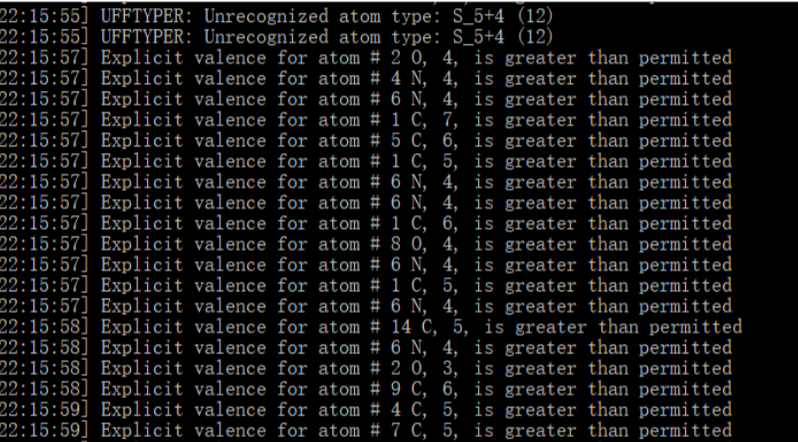
\includegraphics[width=0.75\textwidth]{valencechecks.png}
    \caption{During the run, we can see GCPN doing valence checks for each atom.}
    \label{fig:valencechecks}
\end{figure}

In the original paper, the whole experiment is executed with a 32 core CPU cluster, and training took 8 hours to converge. We therefore could not completely finish training, but still got reasonable results by running a single process for 9.9 hours on normal laptop.

\subsection{Code Source}
An official implementation of ``Graph Convolutional Policy Network for Goal-Directed Molecular Graph Generation" is provided by paper's authors at \textit{https://github.com/bowenliu16/rl\_graph\_generation}.
\section{Results}
The generation of drug-like molecules was trained using the ZINC 250k dataset. We weren’t able to have the process converge, but we were able to keep it running for 9.9 hours, before we terminated the process. The output is a csv file that consists of each iteration the program ran. Each iteration consists of the molecule(s) generated and labeled in the SMILES representation, and several training rewards for each molecule. In this run, we focused on generating molecules with the highest possible penalized logP and QED scores. logP score accounts for synthetic accessibility and QED score indicates druglikeness.

When generating molecules, there are two types of rewards that guide the behavior of the RL agent: domain-specific rewards and intermediate rewards. Domain-specific rewards consist of the combination of final property scores, such as octanol-water partition coefficient (logP), druglikeness, and molecular weight. In addition, it includes the penalization of unrealistic molecules that violate steric strain and zinc functional group rules. Intermediate rewards consist of the stepwise validity rewards and adversarial rewards. For example, if no valency rules are violated then a small positive value is added to the stepwise reward. For the adversarial rewards, the GAN framework is employed to ensure the generated molecules resemble the training set of molecules. The specific rewards indicated in the output file are: \textbf{reward\_valid}, \textbf{reward\_qed}, \textbf{reward\_sa}, \textbf{rew\_env}, \textbf{rew\_d\_step}, \textbf{rew\_d\_final}, \textbf{cur\_ep\_ret}, \textbf{flag\_steric\_filter}, \textbf{flag\_zinc\_filter}, and \textbf{stop}.

\textbf{reward\_valid} has a value of 2 if it passes the 3D conversion check, meaning that there’s no excessive strain on the molecule and it if doesn’t contain any problematic functional groups. (i.e. If flag\_steric\_strain\_filter is TRUE and flag\_zinc\_molecule\_filter is also TRUE, this variable receives a value of 2). Subtract 1 from this score for each filter failed.

\textbf{reward\_qed} is the reward for druglikeness (QED). Its values are between [0,1]. The higher the reward the better, since we are trying to maximize this value. QED stands for the quantitative estimation of drug-likeness. The QED score reflects the underlying distribution of molecular properties, such as topological polar surface area, number of hydrogen bond donors and acceptors and the number of aromatic rings and rotatable bonds.

\textbf{reward\_sa} is the reward for synthetic accessibility. Its values are normalized between [0,1], the higher the better.

\textbf{final\_stat} depends on the reward type (i.e. logP target, QED target, molecular weight target)

\textbf{rew\_env} is a reward value based on an action in the certain environment, given by this formula: env.step(ac)

\textbf{rew\_d\_step} is the discriminator reward from adversarial training on partial molecules, evaluated for each step and summed.

\textbf{rew\_d\_final} is the adversarial reward for the final molecule.

\textbf{cur\_ep\_ret} returns the reward in the current episode, which is the sum of the previous 3 values for all steps in the current episode.

\textbf{flag\_steric\_strain\_filter} is TRUE if there is no excessive steric strain. This is the increase in potential energy of a molecule due to repulsion between electrons in atoms that are not directly bonded to each other. This makes it unlikely for the molecule to be stable in ordinary conditions, thus not generating a realistic molecule.

\textbf{flag\_zinc\_molecule\_filter} is TRUE if the molecule doesn’t possess any problematic and reactive functional groups based on the zinc functional group list.

\textbf{stop} is TRUE if the molecule is complete and doesn’t need any more additions, i.e. passed a final valency check.

\begin{figure}
    \centering
    \begin{subfigure}{0.3\textwidth}
        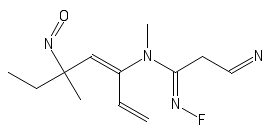
\includegraphics[width=\textwidth]{m1.png}
    \end{subfigure}
    \begin{subfigure}{0.3\textwidth}
        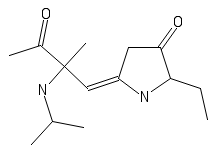
\includegraphics[width=\textwidth]{m3.png}
    \end{subfigure}
    \begin{subfigure}{0.3\textwidth}
        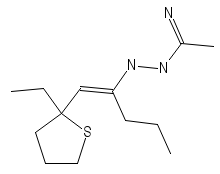
\includegraphics[width=\textwidth]{m4.png}
    \end{subfigure}
    \begin{subfigure}{0.3\textwidth}
        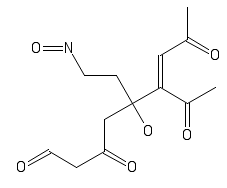
\includegraphics[width=\textwidth]{m5.png}
    \end{subfigure}
    \begin{subfigure}{0.3\textwidth}
        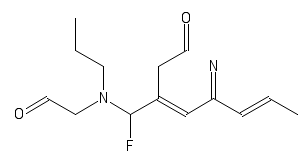
\includegraphics[width=\textwidth]{m6.png}
    \end{subfigure}
    \begin{subfigure}{0.3\textwidth}
        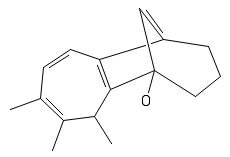
\includegraphics[width=\textwidth]{m7.png}
    \end{subfigure}
    \caption{Stick diagrams of a sample of six brand new molecules generated in the last iteration of training before we terminated the program. These were generated from SMILES strings using the PubChem Sketcher tool. The direct output of the program, including our novel molecules in SMILES format, is given in the attached \texttt{GCPN\_output.csv}.}
    \label{fig:molecules}
\end{figure}





\section{Discussion}
The last iteration that ran was able to generate 11 different molecules that fully satisfied the zinc molecule check and the steric strain check. Therefore, each molecule’s \textbf{reward\_valid} variable is 2. This is not the last iteration of the process, rather the last iteration before we purposely terminated the process before convergence. All other rewards, including reward\_qed and reward\_sa are at least in part iteration-based rewards per molecule, so these values will not necessarily converge to constant values. However, we do expect the QED score and the logP scores to be optimized for the most realistic molecules produced.

It is very difficult to estimate the complete biological impact of a drug-like molecule by simply analyzing it's structure. It is even more difficult to begin with a disease and anticipate the drug structure required to alleviate it. Therefore much of drug research is iterative: small changes are made to the structure of existing drugs and the efficacy of the variants are observed. This is why there are many drug `families' such as the opioids or benzodiazepines: a successful drug was slightly modified in various ways to create new drugs.

To create completely new drug families, however, is an even less straight-forward path. Many thousands of organic molecules from the natural environment are isolated, modified and tested for discovering new potential drugs. Even so, the set of naturally occurring drug-like molecules must only be some small subset of all drug-like molecules. Therefore algorithms such as GCPN present an exciting new avenue for medicine and pharmacology: generating designs for completely new drug candidates that have never been seen before. As the cutting edge in this field, GCPN may pave the way for a new, large, shotgun approach to molecule discovery, synthesis and testing. In the years to come, who knows what diseases may be cured or treated by drugs that were first conceived of in silico by an algorithm such as GCPN?

\newpage
\bibliographystyle{unsrt}
\bibliography{refs}


\end{document}
